
\section{Results}

\begin{figure}
\centering
\begin{tabular}{cc}
\subfloat {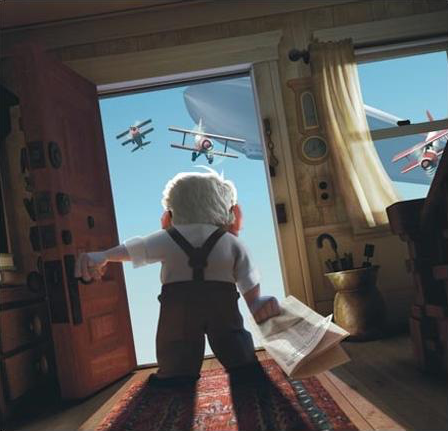
\includegraphics[width=4cm]{images/original_2}} & 
\subfloat {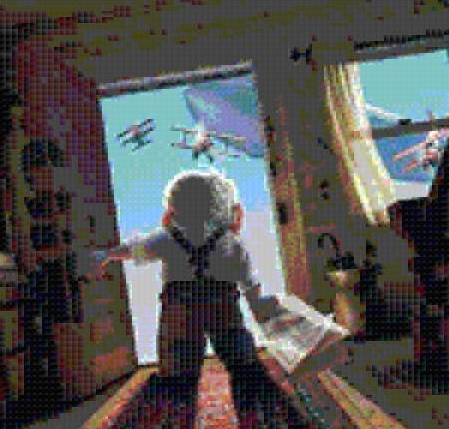
\includegraphics[width=4cm]{images/reconstructed_2}} & 
\end{tabular}
\caption{Visual comparison of original and reconstructed image.}
\label{fig:compare_images}
\end{figure}


We tested the compression algorithm with 100 images which were not in the training set and get a mean error of (......) and a compression rate of (......). 
\newline
Figure~\ref{fig:compare_images} shows an example image before any compression on the left and the reconstructed image after compression on the right. 
\newline
Idea: Test with training directly on image, and compare results with pre-training.

\subsection{Comparison to Baselines}
We compare our solution with two baselines. The first baseline is a compression algorithm based on Gaussian Mixture Models(GMM) and the second algorithm is based on (WHAT IS THE SECOND BASELINE AGAIN?). 
In GMM, .... \newline
Describe baselines here.... \newline
Compare compression rate.... \newline
Compare error....
